% Author: Alejandro Santomé Valverde

\appendix

\refstepcounter{chapter} 
\chapter*{Appendix \thechapter} 
\addcontentsline{toc}{chapter}{Appendix \thechapter}
\markboth{Appendix \thechapter}{}
\label{app:A}

\section{Node equations of the inductive method of a 2x2 network}

Each node represents an input or output port of the $2\times2$ network. The interconnects between
these nodes are modeled by the equations detailed in Figure \ref{fig:appA-link_equations}, where 
$HL$ denoted the scattering matrix of the initial network (e.g., the hexagonal mesh) and $H2$ 
represents the scattering matrix of the newly synthesized circuit.

\begin{figure}[!ht]
    \centering
    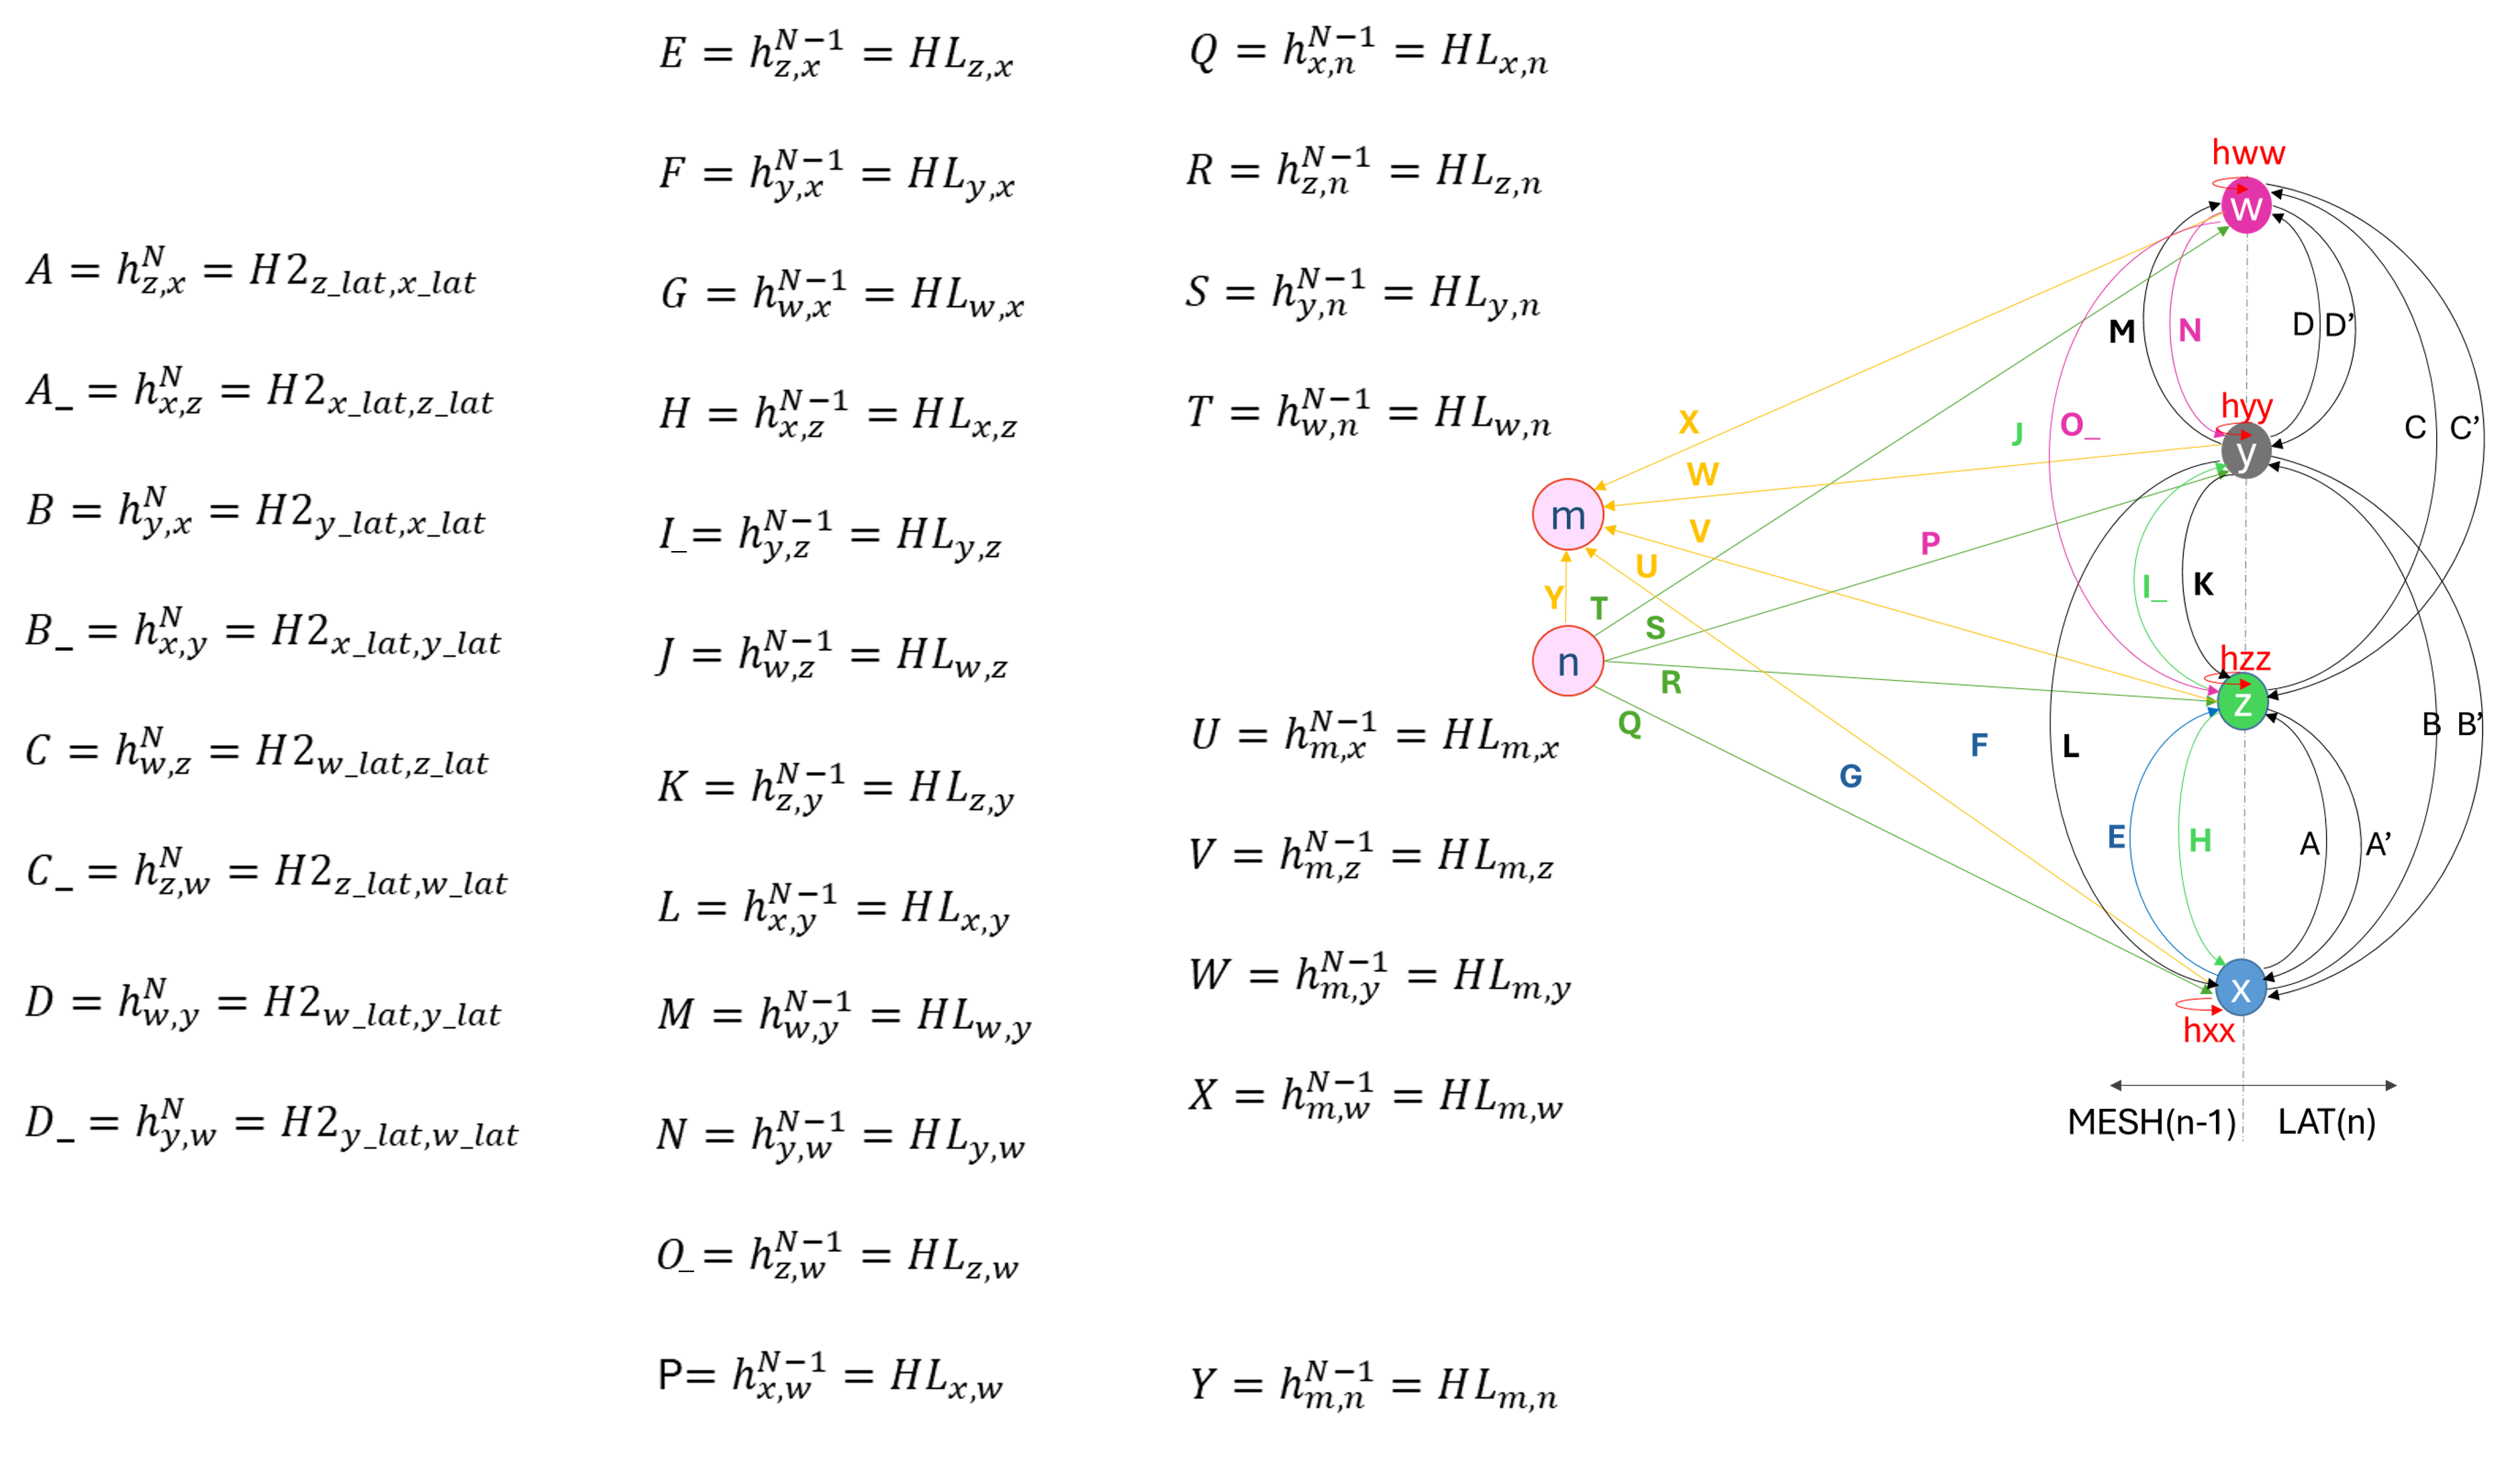
\includegraphics[width=\textwidth]{figures/appA-link_equations.png}
    \caption{Equations (left) of the links connecting the nodes of the signal graph (right) for a
    $2\times2$ ports network.}
    \label{fig:appA-link_equations}
\end{figure}

Figure \ref{fig:appA-node_equations} illustrates all the contributions that enter and exit each 
node, defining the model equations required for the computation of the scattering matrix of the
circuit.

\begin{figure}[!ht]
    \centering
    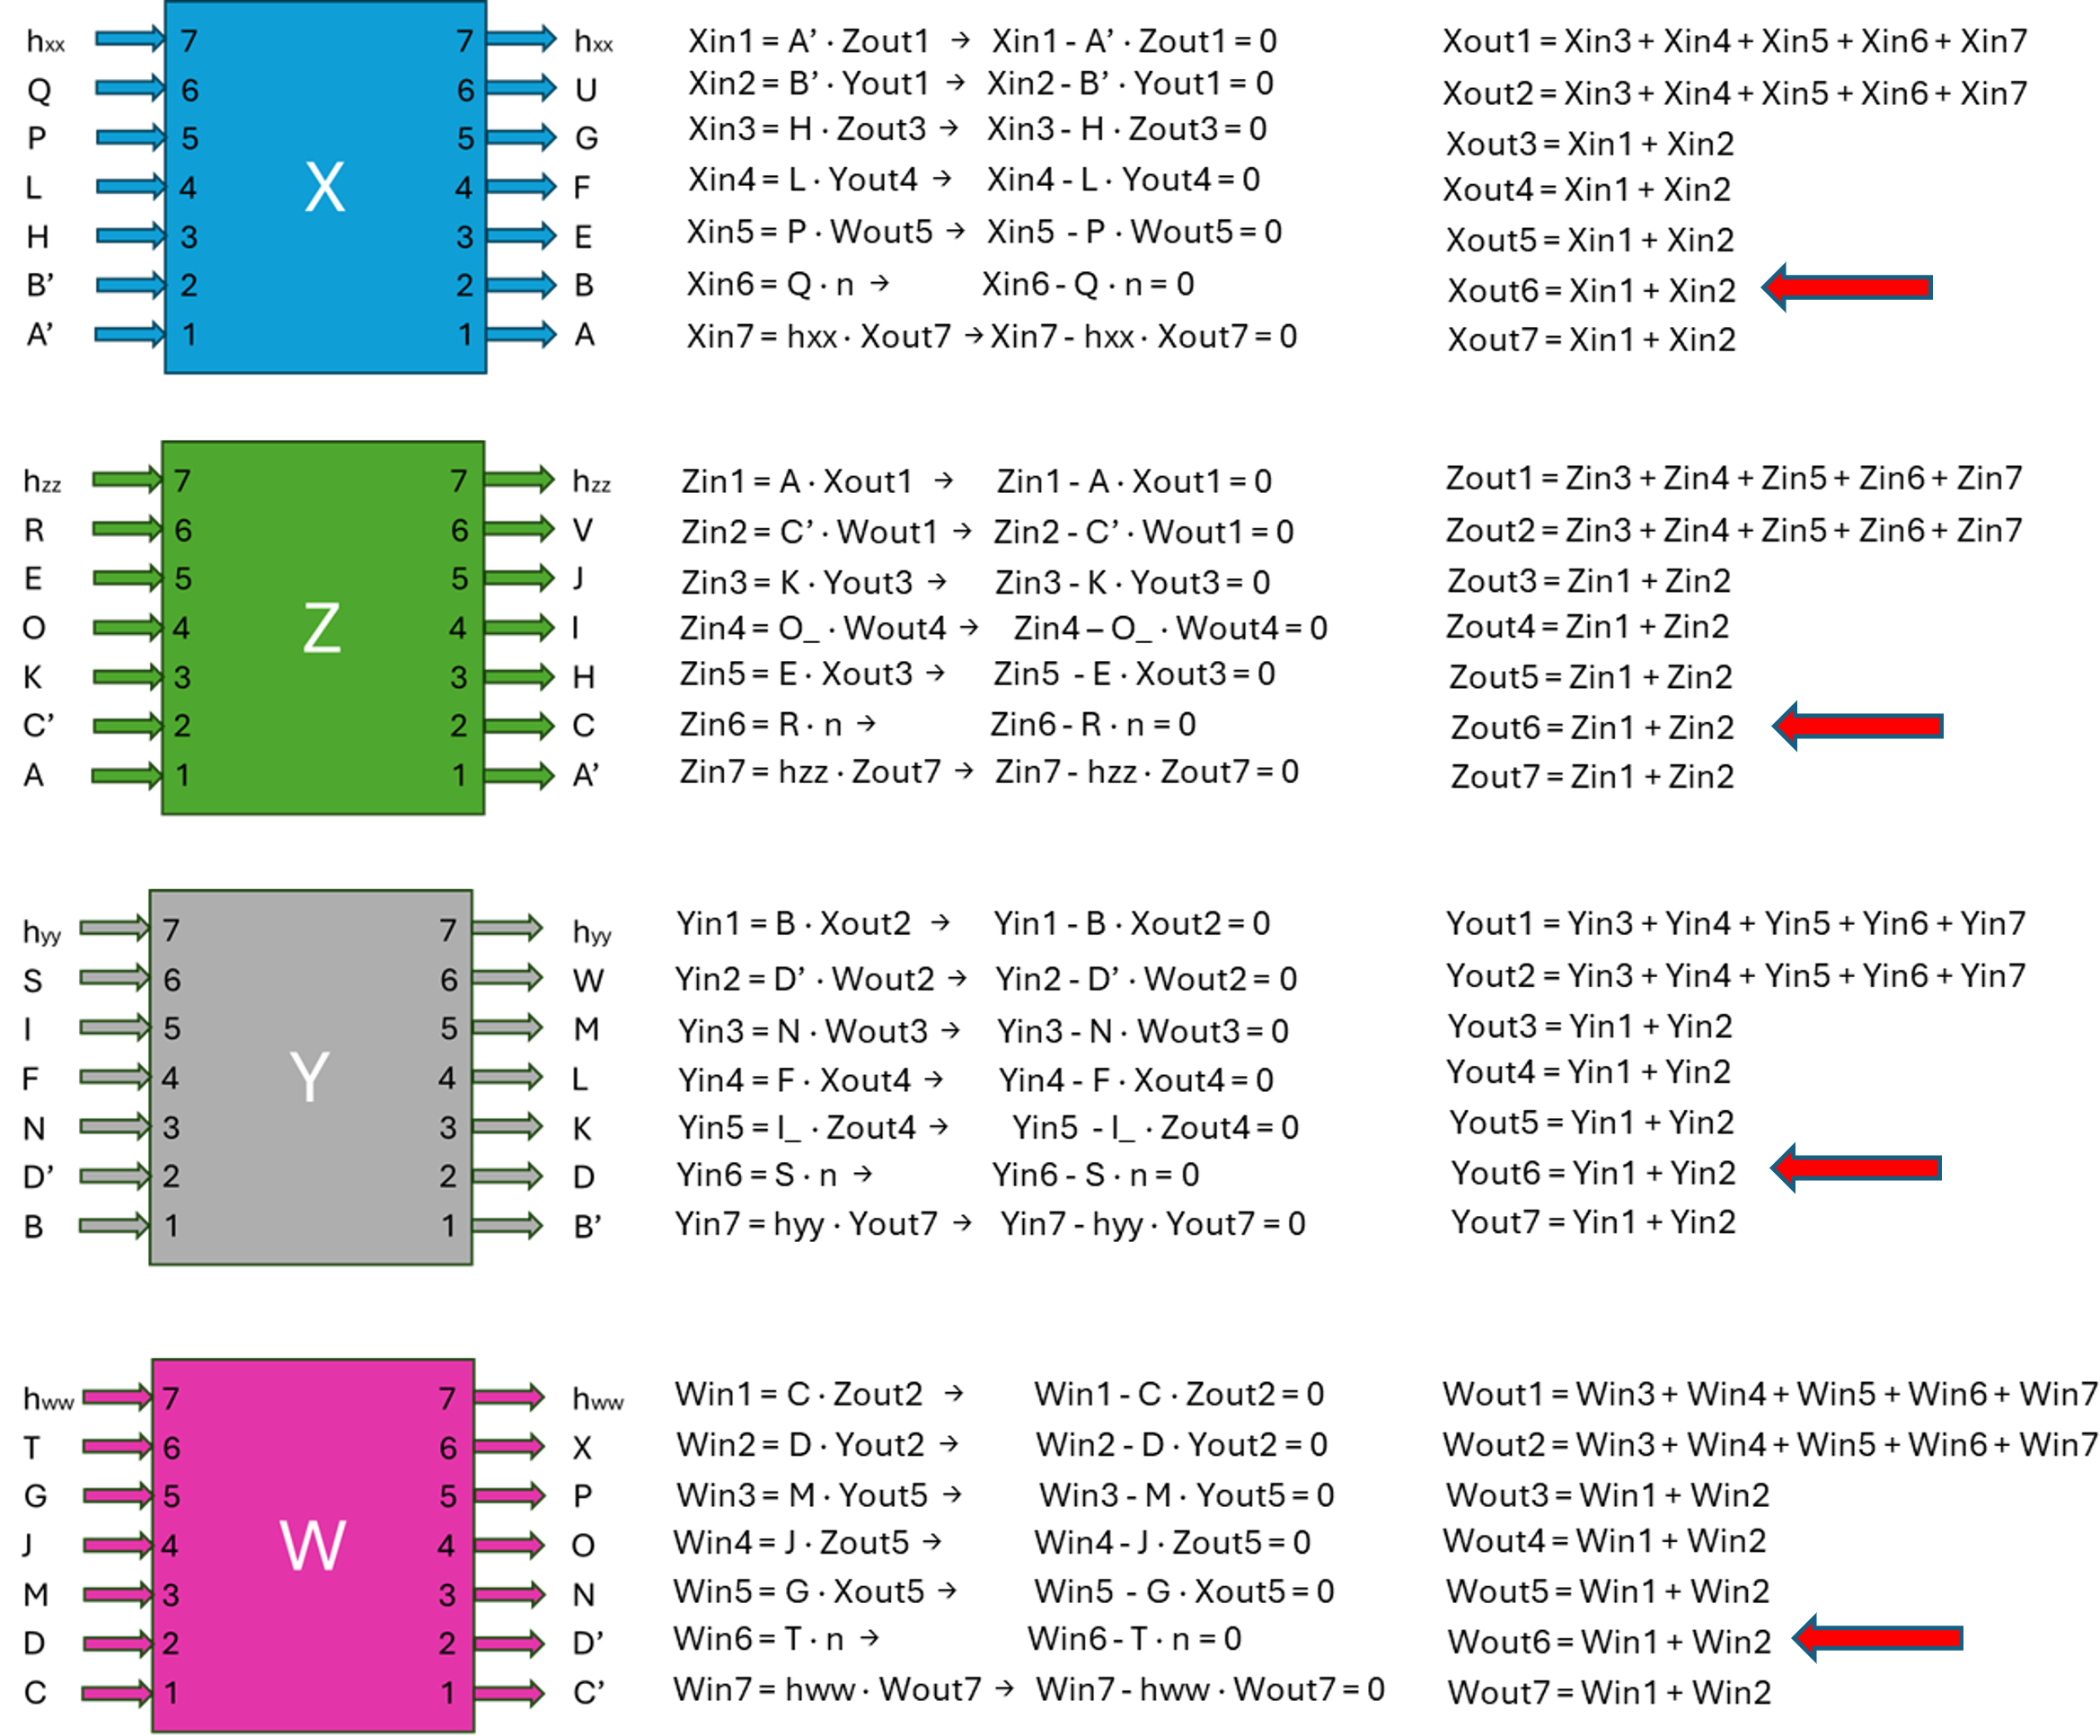
\includegraphics[width=\textwidth]{figures/appA-node_equations.png}
    \caption{Representation of the input and output contributions for each node of a $2\times2$ 
    network using the inductive method. Red arrows represent the links connected to node $m$.}
    \label{fig:appA-node_equations}
\end{figure}

\FloatBarrier

The target result $m$, which is the response of the circuit after connecting the $2\times2$ 
structure, is defined by Equation \ref{app-A:eq_m}, where the highlighted values (red arrows)
of Figure \ref{fig:appA-node_equations} represent the links that are connected to the $m$ node 
(i.e., U, V, W and X).

\begin{equation}
    m = UX_{out_6}+VZ_{out_6}+WY_{out_6}+XW_{out_6} + Y
    \label{app-A:eq_m}
\end{equation}

By using the equations above and computing the response using a matrix solver (e.g., 
\textit{Matlab}), the resulting matrices can be included in the overall response of the 
programmable system.